\documentclass{beamer}
%kdfj
\usetheme[secheader]{Boadilla}
\setbeamertemplate{footline} {
  %\leavevmode%
  \hbox{%
  \begin{beamercolorbox}[wd=.5\paperwidth,ht=2.25ex,dp=1ex,left]{author in head/foot}%
    \usebeamerfont{author in head/foot}\hspace*{2ex}\insertshortauthor~~(adraeger@cern.ch)
  \end{beamercolorbox}%
  \begin{beamercolorbox}[wd=.5\paperwidth,ht=2.25ex,dp=1ex,right]{date in head/foot}%
    \usebeamerfont{date in head/foot}\insertshorttitle,~
    \insertshortdate{}\hspace*{1em}
    \insertframenumber{} / \inserttotalframenumber\hspace*{2ex}
  \end{beamercolorbox}}%
  \vskip0pt%
}
\beamertemplatenavigationsymbolsempty

\usepackage[percent]{overpic}
\usepackage{tikz}
%\usetikzlibrary{positioning,fit,shapes.arrows,shapes.geometric,shapes.misc,shapes.multipart,calc,shadows}
\tikzstyle{every picture}+=[remember picture]
\usepackage{booktabs}
\usepackage{graphicx}
\usepackage{rotating}
\usepackage{wasysym}
\usepackage{marvosym}
\usepackage{amssymb}
\usepackage{xcolor}
\usepackage{tabularx}
\usepackage[normalem]{ulem}
\graphicspath{{../../logo/}{figures/}{../../graphic-common/}}

\input{definitions.tex}
\newcommand{\lib}[1]{\tiny #1}

% Title etc
\vskip2cm
\title[RA2/b Meeting]{Update On Validation of Lepton Efficiencies Using a Tag\&Probe Method}
\subtitle{Lepton Isolation\\ Lepton ID/Reconstruction\\ Isolated Tracks}
\author[Arne-Rasmus~Dr\"ager]{
  Arne-Rasmus~Dr\"ager(Uni Hamburg)
}
\date[July 06, 2015]{July 06, 2015
  \vskip1cm
  \begin{center}
    \includegraphics[height=1.5cm]{Universitaet-Hamburg-Logo.jpg}
    \hskip8cm
    \includegraphics[height=1.5cm]{CMSlogo.jpeg}
  \end{center}
}

% pdflatex packages
\hypersetup{bookmarks=true}
\hypersetup{unicode=false}
\hypersetup{pdftitle={Lost-Lepton}}
\hypersetup{pdfauthor={Arne-Rasmus~Dr\"ager}}


\begin{document}
% ==================================================
% --------------------------------------------------
\begin{frame}
  \titlepage
\end{frame}

\section{Classical Lost-Lepton Method}
\begin{frame}
 \frametitle{Outline}
 \begin{itemize}
  \item Classical Lost-Lepton Method: 
  \begin{itemize}
   \item Isolated track prediction upgrade
  \end{itemize}
  \item Validation of Lepton Efficiencies:
  \begin{itemize}
   \item Electron and muon Tag\&Probe: Iso/Reco validation
   \item Isoalted tracks:
   \begin{itemize}
    \item Isolated e
    \item Isolated $\mu$
    \item Isoalted $\pi$ from $\tau_{had}$
   \end{itemize}
  \end{itemize}
 \end{itemize}
\end{frame}

\begin{frame}
 \begin{block}{}
 \centering
 \Large Classical Lost-Lepton Method: Isolated track bkg reduction closure
 \end{block}
\end{frame}

\subsection{Concept}
\begin{frame}
\frametitle{Rejection of \wpj \& \ttbar events ($W\rightarrow e,\mu$)}
 \begin{center}
\begin{tikzpicture}
    \node[anchor=south west,inner sep=0] (image) at (0,0) {\includegraphics[width=0.75\textwidth]{figures/Sketches/LostLeptonSketch_ll_isotrack.pdf}};
    \begin{scope}[x={(image.south east)},y={(image.north west)}]
%         \draw[red,ultra thick,rounded corners] (0.62,0.65) rectangle (0.78,0.75);
%         \draw[red,ultra thick,rounded corners] (0.60,0.01) rectangle (0.75,0.99); % coordinates unten links(x,y) oben rechts(x,y)
%             \draw[blue,ultra thick,rounded corners] (0.40,0.01) rectangle (0.55,0.99); % coordinates unten links(x,y) oben rechts(x,y)
    \end{scope}
\end{tikzpicture}
 \end{center}
\end{frame}

\begin{frame}
\frametitle{Classical Lost-Lepton Prediciton of Lost Isolated $e,\mu$ events}
 \begin{center}
\begin{tikzpicture}
    \node[anchor=south west,inner sep=0] (image) at (0,0) {\includegraphics[width=0.75\textwidth]{figures/Sketches/LostLeptonSketch_mu_pred_full.pdf}};
    \begin{scope}[x={(image.south east)},y={(image.north west)}]
%         \draw[red,ultra thick,rounded corners] (0.62,0.65) rectangle (0.78,0.75);
%         \draw[red,ultra thick,rounded corners] (0.60,0.01) rectangle (0.75,0.99); % coordinates unten links(x,y) oben rechts(x,y)
%             \draw[blue,ultra thick,rounded corners] (0.40,0.01) rectangle (0.55,0.99); % coordinates unten links(x,y) oben rechts(x,y)
    \end{scope}
\end{tikzpicture}
 \end{center}
\end{frame}


\begin{frame}
\frametitle{Classical Lost-Lepton Procedure}
 \begin{columns}  
 \begin{column}{0.50\textwidth}
\begin{itemize}
 \item The isoalted track veto is an ADDITIONAL reduction of the \ttbar \& \wpj bkg on top of the isolated e,$\mu$ veto!
 \item Combination:
 \begin{itemize}
  \item Apply first iso e,$\mu$ veto. Do full lost-lepton prediction (disregard iso track)
  \item Correct this prediction for further reduction of bkg from isolated tracks
 \end{itemize}

\end{itemize}

   
 \end{column}
 \begin{column}{0.50\textwidth}
\begin{center}
\begin{tikzpicture}
    \node[anchor=south west,inner sep=0] (image) at (0,0) {\includegraphics[width=1.\textwidth]{figures/Sketches/LostLeptonSketch_Prediction_IsoTrackReduction_small.png}};
    \begin{scope}[x={(image.south east)},y={(image.north west)}]
%         \draw[red,ultra thick,rounded corners] (0.62,0.65) rectangle (0.78,0.75);
%         \draw[red,ultra thick,rounded corners] (0.60,0.01) rectangle (0.75,0.99); % coordinates unten links(x,y) oben rechts(x,y)
%             \draw[blue,ultra thick,rounded corners] (0.40,0.01) rectangle (0.55,0.99); % coordinates unten links(x,y) oben rechts(x,y)
    \end{scope}
\end{tikzpicture}
 \end{center}
 \end{column} 
 \end{columns}
 \begin{itemize}
  \item Correction of isolated track reduction is split up in: e, $\mu$ \& $\pi$ tracks
  \item Prediction lost iso. lepton - iso track eff. = Full lost-lepton prediction
 \end{itemize}

\end{frame}
\begin{frame}
 \frametitle{Closure Tests}
\begin{columns}
 \begin{column}{0.50\textwidth}
  \begin{itemize}
   \item Closure before isotrack veto
  \end{itemize}
\begin{tikzpicture}
    \node[anchor=south west,inner sep=0] (image) at (0,0) {\includegraphics[width=1.\textwidth]{figures/lost-lepton_classic/Closure/Baseline/Closure__Bin__MCEx_vs_MuPrMTWDiLep+ElecPrMTWDiLep__Baseline.pdf}};
    \begin{scope}[x={(image.south east)},y={(image.north west)}]
    \end{scope}
\end{tikzpicture}


 \end{column}
 \begin{column}{0.50\textwidth}
  \begin{itemize}
   \item Correcting for iso track veto
  \end{itemize}
\begin{tikzpicture}
    \node[anchor=south west,inner sep=0] (image) at (0,0) {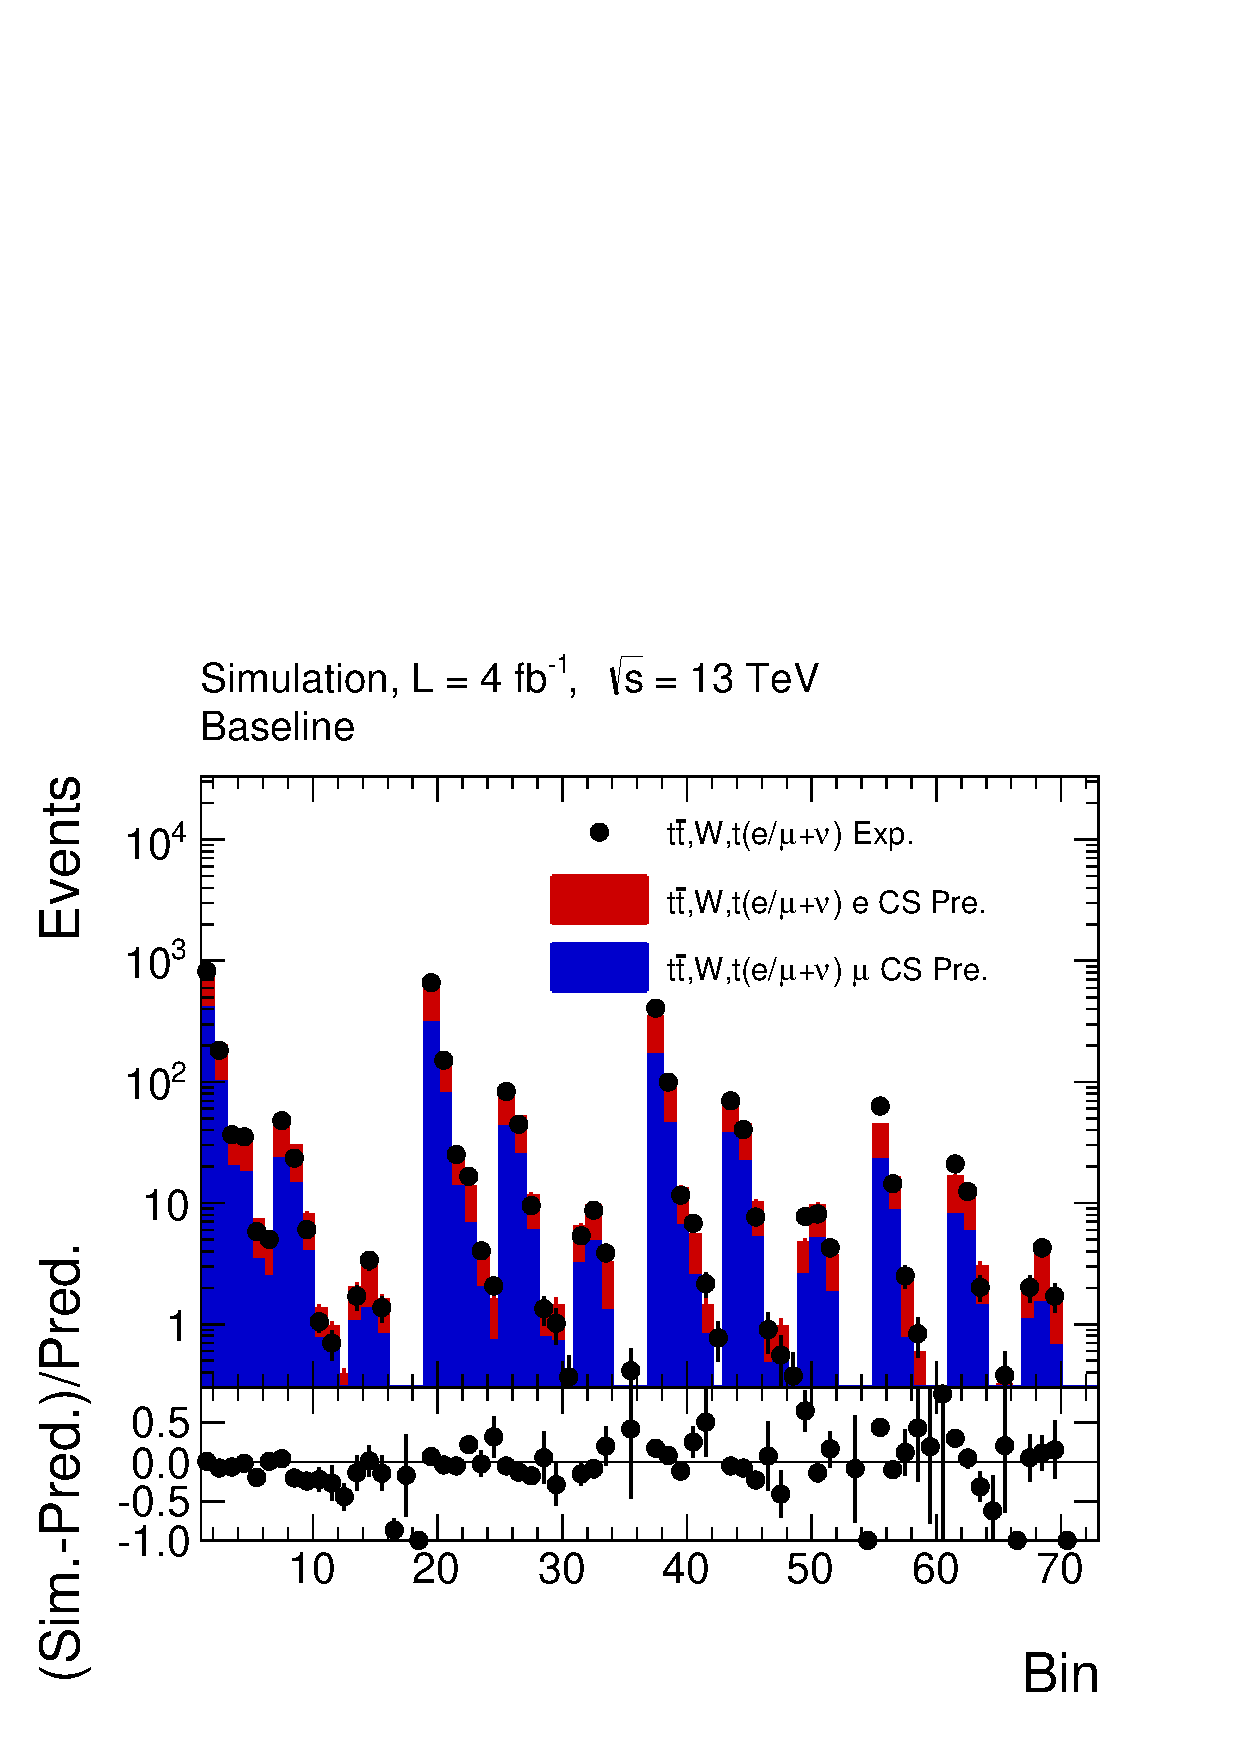
\includegraphics[width=1.\textwidth]{figures/lost-lepton_classic/Closure/Baseline/Closure__Bin__MCEx_vs_MuPrMTWDiLepIsoTrackReduced+ElecPrMTWDiLepIsoTrackReduced__Baseline.pdf}};
    \begin{scope}[x={(image.south east)},y={(image.north west)}]
    \end{scope}
\end{tikzpicture} 
 \end{column}
\end{columns}
\begin{itemize}
 \item The isolated track veto rejects about 40\% of the lost-lepton background! (w/o iso track veto: $2809.8\pm15.7$ with: $1674.1\pm12.0$)
\end{itemize}
\end{frame}

\begin{frame}
 \frametitle{Closer look at rejected events}
\begin{columns}
 \begin{column}{0.50\textwidth}
 \begin{itemize}
  \item w/o iso track veto
 \end{itemize}

\begin{tikzpicture}
    \node[anchor=south west,inner sep=0] (image) at (0,0) {\includegraphics[width=1.\textwidth]{figures/lost-lepton_classic/Composition/Baseline_NoIsoTrack/Composition__Bin__MuIso+MuReco+MuAcc+ElecIso+ElecReco+ElecAcc__Baseline_NoIsoTrack.pdf}};
    \begin{scope}[x={(image.south east)},y={(image.north west)}]
    \end{scope}
\end{tikzpicture}
 \end{column}
 \begin{column}{0.50\textwidth}
  \begin{itemize}
  \item With iso track veto
 \end{itemize}
\begin{tikzpicture}
    \node[anchor=south west,inner sep=0] (image) at (0,0) {\includegraphics[width=1.\textwidth]{figures/lost-lepton_classic/Composition/Baseline/Composition__Bin__MuIso+MuReco+MuAcc+ElecIso+ElecReco+ElecAcc__Baseline.pdf}};
    \begin{scope}[x={(image.south east)},y={(image.north west)}]
    \end{scope}
\end{tikzpicture} 
 \end{column}
\end{columns}
\end{frame}


\begin{frame}
 \frametitle{Closure of Correction Fractions}
\begin{columns}
 \begin{column}{0.50\textwidth}
 \begin{center}
  \begin{tikzpicture}
    \node[anchor=south west,inner sep=0] (image) at (0,0) {\includegraphics[width=.65\textwidth]{figures/lost-lepton_classic/Closure/Baseline/Closure__Bin__MCExIsoTrack_vs_MuPrMTWDiLepIsoTrackReduction+ElecPrMTWDiLepIsoTrackReduction__Baseline.pdf}};
    \begin{scope}[x={(image.south east)},y={(image.north west)}]
    \end{scope}
\end{tikzpicture}
\begin{tikzpicture}
    \node[anchor=south west,inner sep=0] (image) at (0,0) {\includegraphics[width=.65\textwidth]{figures/lost-lepton_classic/Closure/Baseline/Closure__Bin__MCExElecIsoTrack_vs_MuPrMTWDiLepIsoElecTrackReduction+ElecPrMTWDiLepIsoElecTrackReduction__Baseline.pdf}};
    \begin{scope}[x={(image.south east)},y={(image.north west)}]
    \end{scope}
\end{tikzpicture} 
 \end{center}
 \end{column}
 \begin{column}{0.50\textwidth}
 \begin{center}
\begin{tikzpicture}
    \node[anchor=south west,inner sep=0] (image) at (0,0) {\includegraphics[width=.65\textwidth]{figures/lost-lepton_classic/Closure/Baseline/Closure__Bin__MCExMuIsoTrack_vs_MuPrMTWDiLepIsoMuTrackReduction+ElecPrMTWDiLepIsoMuTrackReduction__Baseline.pdf}};
    \begin{scope}[x={(image.south east)},y={(image.north west)}]
    \end{scope}
\end{tikzpicture} 

\begin{tikzpicture}
    \node[anchor=south west,inner sep=0] (image) at (0,0) {\includegraphics[width=.65\textwidth]{figures/lost-lepton_classic/Closure/Baseline/Closure__Bin__MCExPionIsoTrack_vs_MuPrMTWDiLepIsoPionTrackReduction+ElecPrMTWDiLepIsoPionTrackReduction__Baseline.pdf}};
    \begin{scope}[x={(image.south east)},y={(image.north west)}]
    \end{scope}
\end{tikzpicture} 
 \end{center}
 \end{column}
\end{columns}
\end{frame}
  


\begin{frame}
 \frametitle{Efficiencies Parametrization}

 \underline{Muon \& Electron Eff.:}
 \begin{itemize}
  \item Acc.: \HT, \MHT ,\& \NJets
  \item Reco.: \pt, Activity
  \item Iso.: \pt, Activity
  \item \mt: \NJets
  \item Di. lep. CS contribution: \NJets
  \item Di. lep. eff.: \NJets
  \item Iso. $e$ track red.: \MHT, \NJets
  \item Iso. $\mu$ track red.: \MHT, \NJets
  \item Iso. $\pi$ track red.: \MHT, \NJets
 \end{itemize} 
\end{frame}


\begin{frame}
 \begin{block}{}
 \centering
 \Large Tack\&Probe:\\Iso, Reco/ID $e,\mu$ Studies
 \end{block}
\end{frame}

\begin{frame}
\frametitle{Isolateion \& Reconstruction/ID Efficiency Studies}
 \begin{center}
\begin{tikzpicture}
    \node[anchor=south west,inner sep=0] (image) at (0,0) {\includegraphics[width=0.75\textwidth]{figures/Sketches/LostLeptonSketch_mu_pred_full.pdf}};
    \begin{scope}[x={(image.south east)},y={(image.north west)}]
%         \draw[red,ultra thick,rounded corners] (0.62,0.65) rectangle (0.78,0.75);
        \draw[red,ultra thick,rounded corners] (0.60,0.01) rectangle (0.75,0.99); % cordinates unten links(x,y) oben rechts(x,y)
            \draw[blue,ultra thick,rounded corners] (0.40,0.01) rectangle (0.55,0.99); % cordinates unten links(x,y) oben rechts(x,y)
    \end{scope}
\end{tikzpicture}
 \end{center}
\end{frame}

\begin{frame}
 \frametitle{Tag\&Probe Reminder}
 \begin{itemize}
  \item Very established method to study (lepton) efficiencies in Data
  \item Need it to obtain/validate our MC efficiencies in Data
  \end{itemize}
  
  \begin{columns}
 \begin{column}{0.50\textwidth}
 
   \begin{itemize}

  \item Tag\&Probe Concept:
  \begin{itemize}
   \item Select a well understood topology e.g. \Zll evnts
   \item Achieve good ratio of \Zll to other events!
   \item Select Tag object: E.g. well isolated $\mu,e$
   \item Select to be tested object (Probe): Lose defined $\mu,e$. Apply to be tested criteria e.g. isolation to probe object
   \item Compute for passing(p)/failing(f) events invariant mass of di-lepton system (Z mass). 
  \end{itemize}

 \end{itemize}
 \end{column}
  \begin{column}{0.50\textwidth}
\begin{tikzpicture}
    \node[anchor=south west,inner sep=0] (image) at (0,0) {\includegraphics[width=1.\textwidth]{figures/efficiencies/tagandprobe/MuIso_Example_TagAndProbe_Fit.pdf}};
    \begin{scope}[x={(image.south east)},y={(image.north west)}]
%         \draw[red,ultra thick,rounded corners] (0.62,0.65) rectangle (0.78,0.75);
    \end{scope}
\end{tikzpicture}  
\begin{itemize}
 \item Fit passing/failing Z mass distribution: Function: Z resonance \& background shape
 \item $Eff. = p / (p + f)$  
\end{itemize}
  \end{column}
 \end{columns}
\end{frame}

\begin{frame}
 \frametitle{$\mu$ Isolation Efficiencies}
  \begin{columns}

   \begin{column}{0.33\textwidth}
     \begin{itemize}
   \item $\mu$ Iso \ttbar \& \wpj eff.
  \end{itemize}
    \begin{tikzpicture}
    \node[anchor=south west,inner sep=0] (image) at (0,0) {\includegraphics[width=1.\textwidth]{figures/efficiencies/ttbar-wpj/MuIsoPTActivity.pdf}};
    \begin{scope}[x={(image.south east)},y={(image.north west)}]
%         \draw[red,ultra thick,rounded corners] (0.62,0.65) rectangle (0.78,0.75);
%         \draw[red,ultra thick,rounded corners] (0.60,0.01) rectangle (0.75,0.99); % cordinates unten links(x,y) oben rechts(x,y)
    \end{scope}
   \end{tikzpicture}
   \end{column}
   \begin{column}{0.33\textwidth}
   \begin{itemize}
    \item $\mu$ Iso Tag \& Probe eff.
   \end{itemize}

    \begin{tikzpicture}
    \node[anchor=south west,inner sep=0] (image) at (0,0) {\includegraphics[width=1.\textwidth]{figures/efficiencies/tagandprobe/MuIsoTagAndProbeMC.pdf}};
    \begin{scope}[x={(image.south east)},y={(image.north west)}]
%         \draw[red,ultra thick,rounded corners] (0.62,0.65) rectangle (0.78,0.75);
%         \draw[red,ultra thick,rounded corners] (0.60,0.01) rectangle (0.75,0.99); % cordinates unten links(x,y) oben rechts(x,y)
    \end{scope}
   \end{tikzpicture}
   \end{column}
   \begin{column}{0.33\textwidth}
   \begin{itemize}
    \item Ratio: \ttbar \& \wpj / Tag \& Probe eff.
   \end{itemize}

    \begin{tikzpicture}
    \node[anchor=south west,inner sep=0] (image) at (0,0) {\includegraphics[width=1.\textwidth]{figures/efficiencies/tagandprobe/MuIsoPTActivity_ratio.pdf}};
    \begin{scope}[x={(image.south east)},y={(image.north west)}]
%         \draw[red,ultra thick,rounded corners] (0.62,0.65) rectangle (0.78,0.75);
%         \draw[red,ultra thick,rounded corners] (0.60,0.01) rectangle (0.75,0.99); % cordinates unten links(x,y) oben rechts(x,y)
    \end{scope}
   \end{tikzpicture}
   \end{column}
  \end{columns}
\begin{itemize}
 \item Good agreement between \ttbar \& \wpj \& Tag\&Probe $\mu$ isolation efficiencies! 
 \item Tag\&Probe are always slightly above \ttbar \& \wpj eff.
\end{itemize}

\end{frame}


\begin{frame}
 \frametitle{e Isolation Efficiencies}
  \begin{columns}

   \begin{column}{0.33\textwidth}
     \begin{itemize}
   \item e Iso \ttbar \& \wpj eff.
  \end{itemize}
    \begin{tikzpicture}
    \node[anchor=south west,inner sep=0] (image) at (0,0) {\includegraphics[width=1.\textwidth]{figures/efficiencies/ttbar-wpj/ElecIsoPTActivity.pdf}};
    \begin{scope}[x={(image.south east)},y={(image.north west)}]
%         \draw[red,ultra thick,rounded corners] (0.62,0.65) rectangle (0.78,0.75);
%         \draw[red,ultra thick,rounded corners] (0.60,0.01) rectangle (0.75,0.99); % cordinates unten links(x,y) oben rechts(x,y)
    \end{scope}
   \end{tikzpicture}
   \end{column}
   \begin{column}{0.33\textwidth}
   \begin{itemize}
    \item e Iso Tag \& Probe eff.
   \end{itemize}

    \begin{tikzpicture}
    \node[anchor=south west,inner sep=0] (image) at (0,0) {\includegraphics[width=1.\textwidth]{figures/efficiencies/tagandprobe/ElecIsoTagAndProbeMC.pdf}};
    \begin{scope}[x={(image.south east)},y={(image.north west)}]
%         \draw[red,ultra thick,rounded corners] (0.62,0.65) rectangle (0.78,0.75);
%         \draw[red,ultra thick,rounded corners] (0.60,0.01) rectangle (0.75,0.99); % cordinates unten links(x,y) oben rechts(x,y)
    \end{scope}
   \end{tikzpicture}
   \end{column}
   \begin{column}{0.33\textwidth}
   \begin{itemize}
    \item Ratio: \ttbar \& \wpj / Tag \& Probe eff.
   \end{itemize}

    \begin{tikzpicture}
    \node[anchor=south west,inner sep=0] (image) at (0,0) {\includegraphics[width=1.\textwidth]{figures/efficiencies/tagandprobe/ElecIsoPTActivity_ratio.pdf}};
    \begin{scope}[x={(image.south east)},y={(image.north west)}]
%         \draw[red,ultra thick,rounded corners] (0.62,0.65) rectangle (0.78,0.75);
%         \draw[red,ultra thick,rounded corners] (0.60,0.01) rectangle (0.75,0.99); % cordinates unten links(x,y) oben rechts(x,y)
    \end{scope}
   \end{tikzpicture}
   \end{column}
  \end{columns}
\begin{itemize}
 \item Good agreement between \ttbar \& \wpj \& Tag\&Probe e isolation efficiencies! 
 \item Tag\&Probe are always slightly above \ttbar \& \wpj eff.
\end{itemize}

\end{frame}

\begin{frame}
 \frametitle{Reconstruction \& ID validation}
 
   \begin{columns}
 \begin{column}{0.50\textwidth}
 
   \begin{itemize}
  \item We compute our combined reco/ID eff using gen information:
  \begin{itemize}
   \item Reco/ID Eff.: Select events with prompt lepton $\rightarrow$ Ask for $\pt>10\gev$ \& $|\eta|<2.5(2.4)$ (on gen) $\rightarrow$ try to match well reconstructed and ID lepton (on reco level) $eff.=p/(p+f)$
  \end{itemize}
  \item Tag\&Probe Difficultiy: 
  \item No gen info available. Test object selected on reco level. Most basic object desirable (avoid gab see above).
  \end{itemize}
 \end{column}
  \begin{column}{0.50\textwidth}
\begin{tikzpicture}
    \node[anchor=south west,inner sep=0] (image) at (0,0) {\includegraphics[width=1.\textwidth]{figures/efficiencies/tagandprobe/MuIso_Example_TagAndProbe_Fit.pdf}};
    \begin{scope}[x={(image.south east)},y={(image.north west)}]
%         \draw[red,ultra thick,rounded corners] (0.62,0.65) rectangle (0.78,0.75);
    \end{scope}
\end{tikzpicture}  
\begin{itemize}
 \item BUT need to keep ratio Z mass signal over bkg reasonable for fit! Especially in failing collection!
 \item $Eff. = p / (p + f)$  
\end{itemize}
  \end{column}
 \end{columns}
\end{frame}
\begin{frame}
 \frametitle{Reconstruction \& ID Tag\&Probe Setup}
 
 Setup:
 \begin{itemize}
  \item Tag: Isolated $\mu/e$
  \item Probe:
  \begin{itemize}
   \item $\mu$: miniAOD slimmedMuon; Gap: Missing muons within acceptance ($\pt>10\gev$ \& $|\eta|<2.4$)  that are NOT slimmedMuons\\ (most basic: tracker muons)
   \item $e$: miniAOD slimmedPhoton; Gap: Missing electrons within acceptance ($\pt>10\gev$ \& $|\eta|<2.5$) that are NOT Photons (especially in high Activity region) (most basic: superclusters)
  \end{itemize}
 \end{itemize}
\end{frame}
\begin{frame}
 \frametitle{$\mu$ Reconstruction/ID Efficiencies}
  \begin{columns}

   \begin{column}{0.33\textwidth}
     \begin{itemize}
   \item $\mu$ Reco/ID \ttbar \& \wpj eff.
  \end{itemize}
    \begin{tikzpicture}
    \node[anchor=south west,inner sep=0] (image) at (0,0) {\includegraphics[width=1.\textwidth]{figures/efficiencies/ttbar-wpj/MuRecoPTActivity.pdf}};
    \begin{scope}[x={(image.south east)},y={(image.north west)}]
%         \draw[red,ultra thick,rounded corners] (0.62,0.65) rectangle (0.78,0.75);
%         \draw[red,ultra thick,rounded corners] (0.60,0.01) rectangle (0.75,0.99); % cordinates unten links(x,y) oben rechts(x,y)
    \end{scope}
   \end{tikzpicture}
   \end{column}
   \begin{column}{0.33\textwidth}
   \begin{itemize}
    \item $\mu$ Reco/ID Tag \& Probe eff.
   \end{itemize}

    \begin{tikzpicture}
    \node[anchor=south west,inner sep=0] (image) at (0,0) {\includegraphics[width=1.\textwidth]{figures/efficiencies/tagandprobe/MuRecoTagAndProbeMC.pdf}};
    \begin{scope}[x={(image.south east)},y={(image.north west)}]
%         \draw[red,ultra thick,rounded corners] (0.62,0.65) rectangle (0.78,0.75);
%         \draw[red,ultra thick,rounded corners] (0.60,0.01) rectangle (0.75,0.99); % cordinates unten links(x,y) oben rechts(x,y)
    \end{scope}
   \end{tikzpicture}
   \end{column}
   \begin{column}{0.33\textwidth}
   \begin{itemize}
    \item Ratio: \ttbar \& \wpj / Tag \& Probe eff.
   \end{itemize}

    \begin{tikzpicture}
    \node[anchor=south west,inner sep=0] (image) at (0,0) {\includegraphics[width=1.\textwidth]{figures/efficiencies/tagandprobe/MuRecoPTActivity_ratio.pdf}};
    \begin{scope}[x={(image.south east)},y={(image.north west)}]
%         \draw[red,ultra thick,rounded corners] (0.62,0.65) rectangle (0.78,0.75);
%         \draw[red,ultra thick,rounded corners] (0.60,0.01) rectangle (0.75,0.99); % cordinates unten links(x,y) oben rechts(x,y)
    \end{scope}
   \end{tikzpicture}
   \end{column}
  \end{columns}
\begin{itemize}
 \item Overall the expected higher efficiencies can be observed in Tag\&Probe due to the gab of probe object (slimmedMuon) and all muons within acceptance
\end{itemize}

\end{frame}


\begin{frame}
 \frametitle{e Reconstruction/ID Efficiencies}
  \begin{columns}

   \begin{column}{0.33\textwidth}
     \begin{itemize}
   \item e Reco/ID \ttbar \& \wpj eff.
  \end{itemize}
    \begin{tikzpicture}
    \node[anchor=south west,inner sep=0] (image) at (0,0) {\includegraphics[width=1.\textwidth]{figures/efficiencies/ttbar-wpj/ElecRecoPTActivity.pdf}};
    \begin{scope}[x={(image.south east)},y={(image.north west)}]
%         \draw[red,ultra thick,rounded corners] (0.62,0.65) rectangle (0.78,0.75);
%         \draw[red,ultra thick,rounded corners] (0.60,0.01) rectangle (0.75,0.99); % cordinates unten links(x,y) oben rechts(x,y)
    \end{scope}
   \end{tikzpicture}
   \end{column}
   \begin{column}{0.33\textwidth}
   \begin{itemize}
    \item e Reco/ID Tag \& Probe eff.
   \end{itemize}

    \begin{tikzpicture}
    \node[anchor=south west,inner sep=0] (image) at (0,0) {\includegraphics[width=1.\textwidth]{figures/efficiencies/tagandprobe/ElecRecoTagAndProbeMC.pdf}};
    \begin{scope}[x={(image.south east)},y={(image.north west)}]
%         \draw[red,ultra thick,rounded corners] (0.62,0.65) rectangle (0.78,0.75);
%         \draw[red,ultra thick,rounded corners] (0.60,0.01) rectangle (0.75,0.99); % cordinates unten links(x,y) oben rechts(x,y)
    \end{scope}
   \end{tikzpicture}
   \end{column}
   \begin{column}{0.33\textwidth}
   \begin{itemize}
    \item Ratio: \ttbar \& \wpj / Tag \& Probe eff.
   \end{itemize}

    \begin{tikzpicture}
    \node[anchor=south west,inner sep=0] (image) at (0,0) {\includegraphics[width=1.\textwidth]{figures/efficiencies/tagandprobe/ElecRecoPTActivity_ratio.pdf}};
    \begin{scope}[x={(image.south east)},y={(image.north west)}]
%         \draw[red,ultra thick,rounded corners] (0.62,0.65) rectangle (0.78,0.75);
%         \draw[red,ultra thick,rounded corners] (0.60,0.01) rectangle (0.75,0.99); % cordinates unten links(x,y) oben rechts(x,y)
    \end{scope}
   \end{tikzpicture}
   \end{column}
  \end{columns}
\begin{itemize}
 \item At high $\pt$ to Activity ratio good agreement. Increasing activity increases probability to lose already probe object (photon) biases to higher eff in Tag\&Probe. Also $\pt$ threshold of Probe objects at 15\gev.
\end{itemize}

\end{frame}


\begin{frame}
 \begin{block}{}
 \centering
 \Large Tack\&Probe:\\Isolated $e,\mu,\pi$ tracks Studies
 \end{block}
\end{frame}


\subsection{Concept}
\begin{frame}
\frametitle{Iso Track Reduction}
 \begin{center}
\begin{tikzpicture}
    \node[anchor=south west,inner sep=0] (image) at (0,0) {\includegraphics[width=0.5\textwidth]{figures/Sketches/LostLeptonSketch_Prediction_IsoTrackReduction_small.png}};
    \begin{scope}[x={(image.south east)},y={(image.north west)}]
%         \draw[red,ultra thick,rounded corners] (0.62,0.65) rectangle (0.78,0.75);
%         \draw[red,ultra thick,rounded corners] (0.60,0.01) rectangle (0.75,0.99); % coordinates unten links(x,y) oben rechts(x,y)
%             \draw[blue,ultra thick,rounded corners] (0.40,0.01) rectangle (0.55,0.99); % coordinates unten links(x,y) oben rechts(x,y)
    \end{scope}
\end{tikzpicture}
 \end{center}
 \begin{itemize}
  \item Correction factor is split up in: $\epsilon_{track} = \epsilon_{\mu} +\epsilon_{e} +\epsilon_{\pi} $ where $\epsilon_{\pi}$ contains $\mu/e$ that fail the pdgID assignment from PF algorithm
  \item Study these efficiencies using Tag and Probe
 \end{itemize}
\end{frame}
\begin{frame}
 \frametitle{Tag\&Probe Setup}
\begin{itemize}
 \item Muon, Electron Tracks:
 \begin{itemize}
  \item Charged PFCand, $\pt>5 \gev, |\eta|<2.5$, $\mt<100 \gev$, ask for pdgID=11,13
  \item Iso: $\Sigma ( \pt\text(Tracks)\Delta R<0.3 )/(\pt Track) < 0.2$ (with $dz<0.1$)
 \end{itemize}
 \item Pion Tracks:
 \begin{itemize}
  \item Charged PFCand, $\pt>10 \gev, |\eta|<2.5$, $\mt<100 \gev$, ask for pdgID=211
  \item Iso: $\Sigma ( \pt\text(Tracks)\Delta R<0.3 )/(\pt Track) < 0.1$ (with $dz<0.1$)
 \end{itemize}
 \end{itemize}

 
\end{frame}

\begin{frame}
 \frametitle{Where do we apply the isolated Track veto?}
 \begin{itemize}
  \item Isolated track veto is applied on top of isolated lepton veto
  \begin{itemize}
   \item We are interested in the fraction of lost isolated electron and muon events which are selected by the isolated track veto
  \end{itemize}
  \item Rejection efficiency derived on simulated \ttbar \& \wpj events $\rightarrow$ applied to data
  \item Need to validate in data using Tag\&Probe
  \item Tag objects: Well isolated $\mu/e$
  \item Probe objects: Tracks within acceptance cuts with pdgID of $\mu/e$ applied by PF algorithm. Leaving two gabs:
  \begin{itemize}
   \item Can not account of  $\mu/e$  failing pdgID assignment
   \item Those events might become isolated $\pi$ tracks (20\%).
  \end{itemize}
  \item Check similarity of $\mu_{gen}\rightarrow \mu_{Isotrack}$ \& $\mu_{gen}\rightarrow \pi_{Isotrack}$ (same for e)
  \item Check similarity of $ \tau_{had gen}\rightarrow \pi_{Isotrack}$ for $\tau\rightarrow\pi^{\pm}+\nu_{tau}$ and $\tau\rightarrow\pi^{\pm}+\nu_{tau}+x\pi^{0}$
 \end{itemize}
\end{frame}
\begin{frame}
 \frametitle{Transfer from \wpj \& \ttbar to DY events}
 \begin{itemize}
  \item Need to account for kinematic differences in efficiencies parametrization: Use \pt Activity around tracks
  \begin{itemize}
   \item Problem: $\mu \& e$ tracks defined $\pt>5 \gev$ $\mu \& e$ CS only defined $\pt>10 \gev$
  \end{itemize}
  \item Isolated tracks selection: $\mt<100 \gev$ Not defined in \Zll
  \begin{itemize}
   \item Subtract tag lepton \pt from MET to emulate $\nu$
  \end{itemize}
 \end{itemize}
\begin{center}
\begin{overpic}[width=.40\textwidth]{figures/efficiencies/tagandprobe/TagAndProbe__MTW__MuIso_vs_MuIsoMTWClean__Baseline.pdf}      %\put(18,36.2){\color{red}\line(1,0){75}}
      \end{overpic}
\begin{overpic}[width=.40\textwidth]{figures/efficiencies/tagandprobe/TagAndProbe__MTW__ElecIso_vs_ElecIsoMTWClean__Baseline.pdf}      %\put(18,36.2){\color{red}\line(1,0){75}}
      \end{overpic} 
\end{center}


\end{frame}



\begin{frame}
 \frametitle{Comparison \ttbar \& \wpj vs Tag \& Probe Efficiencies}
  \begin{columns}

   \begin{column}{0.33\textwidth}
     \begin{itemize}
   \item $\mu$ track \ttbar \& \wpj eff. (truth info.)
  \end{itemize}
    \begin{tikzpicture}
    \node[anchor=south west,inner sep=0] (image) at (0,0) {\includegraphics[width=1.\textwidth]{figures/efficiencies/ttbar-wpj/MuIsoTrackGenMuReductionPTActivity.pdf}};
    \begin{scope}[x={(image.south east)},y={(image.north west)}]
%         \draw[red,ultra thick,rounded corners] (0.62,0.65) rectangle (0.78,0.75);
%         \draw[red,ultra thick,rounded corners] (0.60,0.01) rectangle (0.75,0.99); % cordinates unten links(x,y) oben rechts(x,y)
    \end{scope}
   \end{tikzpicture}
   \end{column}
   \begin{column}{0.33\textwidth}
   \begin{itemize}
    \item $\mu$ track DY eff. \\(Tag\&Probe)
   \end{itemize}

    \begin{tikzpicture}
    \node[anchor=south west,inner sep=0] (image) at (0,0) {\includegraphics[width=1.\textwidth]{figures/efficiencies/tagandprobe/MuTrackTagAndProbeMC.pdf}};
    \begin{scope}[x={(image.south east)},y={(image.north west)}]
%         \draw[red,ultra thick,rounded corners] (0.62,0.65) rectangle (0.78,0.75);
%         \draw[red,ultra thick,rounded corners] (0.60,0.01) rectangle (0.75,0.99); % cordinates unten links(x,y) oben rechts(x,y)
    \end{scope}
   \end{tikzpicture}
   \end{column}
           \begin{column}{0.33\textwidth}
   \begin{itemize}
    \item Ratio: \ttbar \& \wpj / Tag\&Probe
   \end{itemize}

    \begin{tikzpicture}
     \node[anchor=south west,inner sep=0] (image) at (0,0) {\includegraphics[width=1.\textwidth]{figures/efficiencies/tagandprobe/MuIsoTrackGenMuPTActivity_ratio.pdf}};
    \begin{scope}[x={(image.south east)},y={(image.north west)}]
%         \draw[red,ultra thick,rounded corners] (0.62,0.65) rectangle (0.78,0.75);
%         \draw[red,ultra thick,rounded corners] (0.60,0.01) rectangle (0.75,0.99); % cordinates unten links(x,y) oben rechts(x,y)
    \end{scope}
   \end{tikzpicture}
   \end{column}
  \end{columns}
  \begin{itemize}
   \item Rather good agreement over the full \pt and Activity range
   \item Good agreement in the important $5\leq\pt\leq10\gev$ region
  \end{itemize}


\end{frame}



\begin{frame}
 \frametitle{Comparison \ttbar \& \wpj vs Tag \& Probe Efficiencies}
  \begin{columns}

   \begin{column}{0.33\textwidth}
     \begin{itemize}
   \item e track \ttbar \& \wpj eff. (truth info.)
  \end{itemize}
    \begin{tikzpicture}
    \node[anchor=south west,inner sep=0] (image) at (0,0) {\includegraphics[width=1.\textwidth]{figures/efficiencies/ttbar-wpj/ElecIsoTrackGenElecReductionPTActivity.pdf}};
    \begin{scope}[x={(image.south east)},y={(image.north west)}]
%         \draw[red,ultra thick,rounded corners] (0.62,0.65) rectangle (0.78,0.75);
%         \draw[red,ultra thick,rounded corners] (0.60,0.01) rectangle (0.75,0.99); % cordinates unten links(x,y) oben rechts(x,y)
    \end{scope}
   \end{tikzpicture}
   \end{column}
   \begin{column}{0.33\textwidth}
   \begin{itemize}
    \item e track DY eff. \\(Tag\&Probe)
   \end{itemize}

    \begin{tikzpicture}
    \node[anchor=south west,inner sep=0] (image) at (0,0) {\includegraphics[width=1.\textwidth]{figures/efficiencies/tagandprobe/ElecTrackTagAndProbeMC.pdf}};
    \begin{scope}[x={(image.south east)},y={(image.north west)}]
%         \draw[red,ultra thick,rounded corners] (0.62,0.65) rectangle (0.78,0.75);
%         \draw[red,ultra thick,rounded corners] (0.60,0.01) rectangle (0.75,0.99); % cordinates unten links(x,y) oben rechts(x,y)
    \end{scope}
   \end{tikzpicture}
   \end{column}
           \begin{column}{0.33\textwidth}
   \begin{itemize}
    \item Ratio: \ttbar \& \wpj / Tag\&Probe
   \end{itemize}

    \begin{tikzpicture}
     \node[anchor=south west,inner sep=0] (image) at (0,0) {\includegraphics[width=1.\textwidth]{figures/efficiencies/tagandprobe/ElecIsoTrackGenElecPTActivity_ratio.pdf}};
    \begin{scope}[x={(image.south east)},y={(image.north west)}]
%         \draw[red,ultra thick,rounded corners] (0.62,0.65) rectangle (0.78,0.75);
%         \draw[red,ultra thick,rounded corners] (0.60,0.01) rectangle (0.75,0.99); % cordinates unten links(x,y) oben rechts(x,y)
    \end{scope}
   \end{tikzpicture}
   \end{column}
  \end{columns}
  \begin{itemize}
   \item Rather good agreement over the full \pt and Activity range
   \item Reasonable agreement in the important $5\leq\pt\leq10\gev$ region
  \end{itemize}
\end{frame}




% \begin{frame}
%  \frametitle{Iso track reduction by component 1}
%  \begin{overpic}[width=.40\textwidth]{figures/efficiencies/ttbar-wpj/IsoTrackReductionPTActivity.pdf}      %\put(18,36.2){\color{red}\line(1,0){75}}
%       \end{overpic}\\
%  \begin{overpic}[width=.32\textwidth]{figures/efficiencies/ttbar-wpj/MuIsoTrackReductionPTActivity.pdf}      %\put(18,36.2){\color{red}\line(1,0){75}}
%       \end{overpic}
%  \begin{overpic}[width=.32\textwidth]{figures/efficiencies/ttbar-wpj/ElecIsoTrackReductionPTActivity.pdf}      %\put(18,36.2){\color{red}\line(1,0){75}}
%       \end{overpic}
%  \begin{overpic}[width=.32\textwidth]{figures/efficiencies/ttbar-wpj/PionIsoTrackReductionPTActivity.pdf}      %\put(18,36.2){\color{red}\line(1,0){75}}
%       \end{overpic}
% \end{frame}



\begin{frame}
 \begin{block}{}
 \centering
 \Large Backup
 \end{block}
\end{frame}





% --------------------------------------------------

\setcounter{framenumber}{26}

\end{document}

